\documentclass[tikz,border=10pt]{standalone}
\usepackage{tikz}
\usetikzlibrary{shapes,arrows,positioning,decorations.pathreplacing,backgrounds,fit,calc}
\usepackage{xcolor}

% Define colors
\definecolor{frontend}{RGB}{97, 218, 251}
\definecolor{backend}{RGB}{40, 167, 69}
\definecolor{database}{RGB}{16, 142, 233}
\definecolor{security}{RGB}{220, 53, 69}
\definecolor{cache}{RGB}{255, 193, 7}
\definecolor{audit}{RGB}{108, 117, 125}
\definecolor{external}{RGB}{111, 66, 193}

\begin{document}
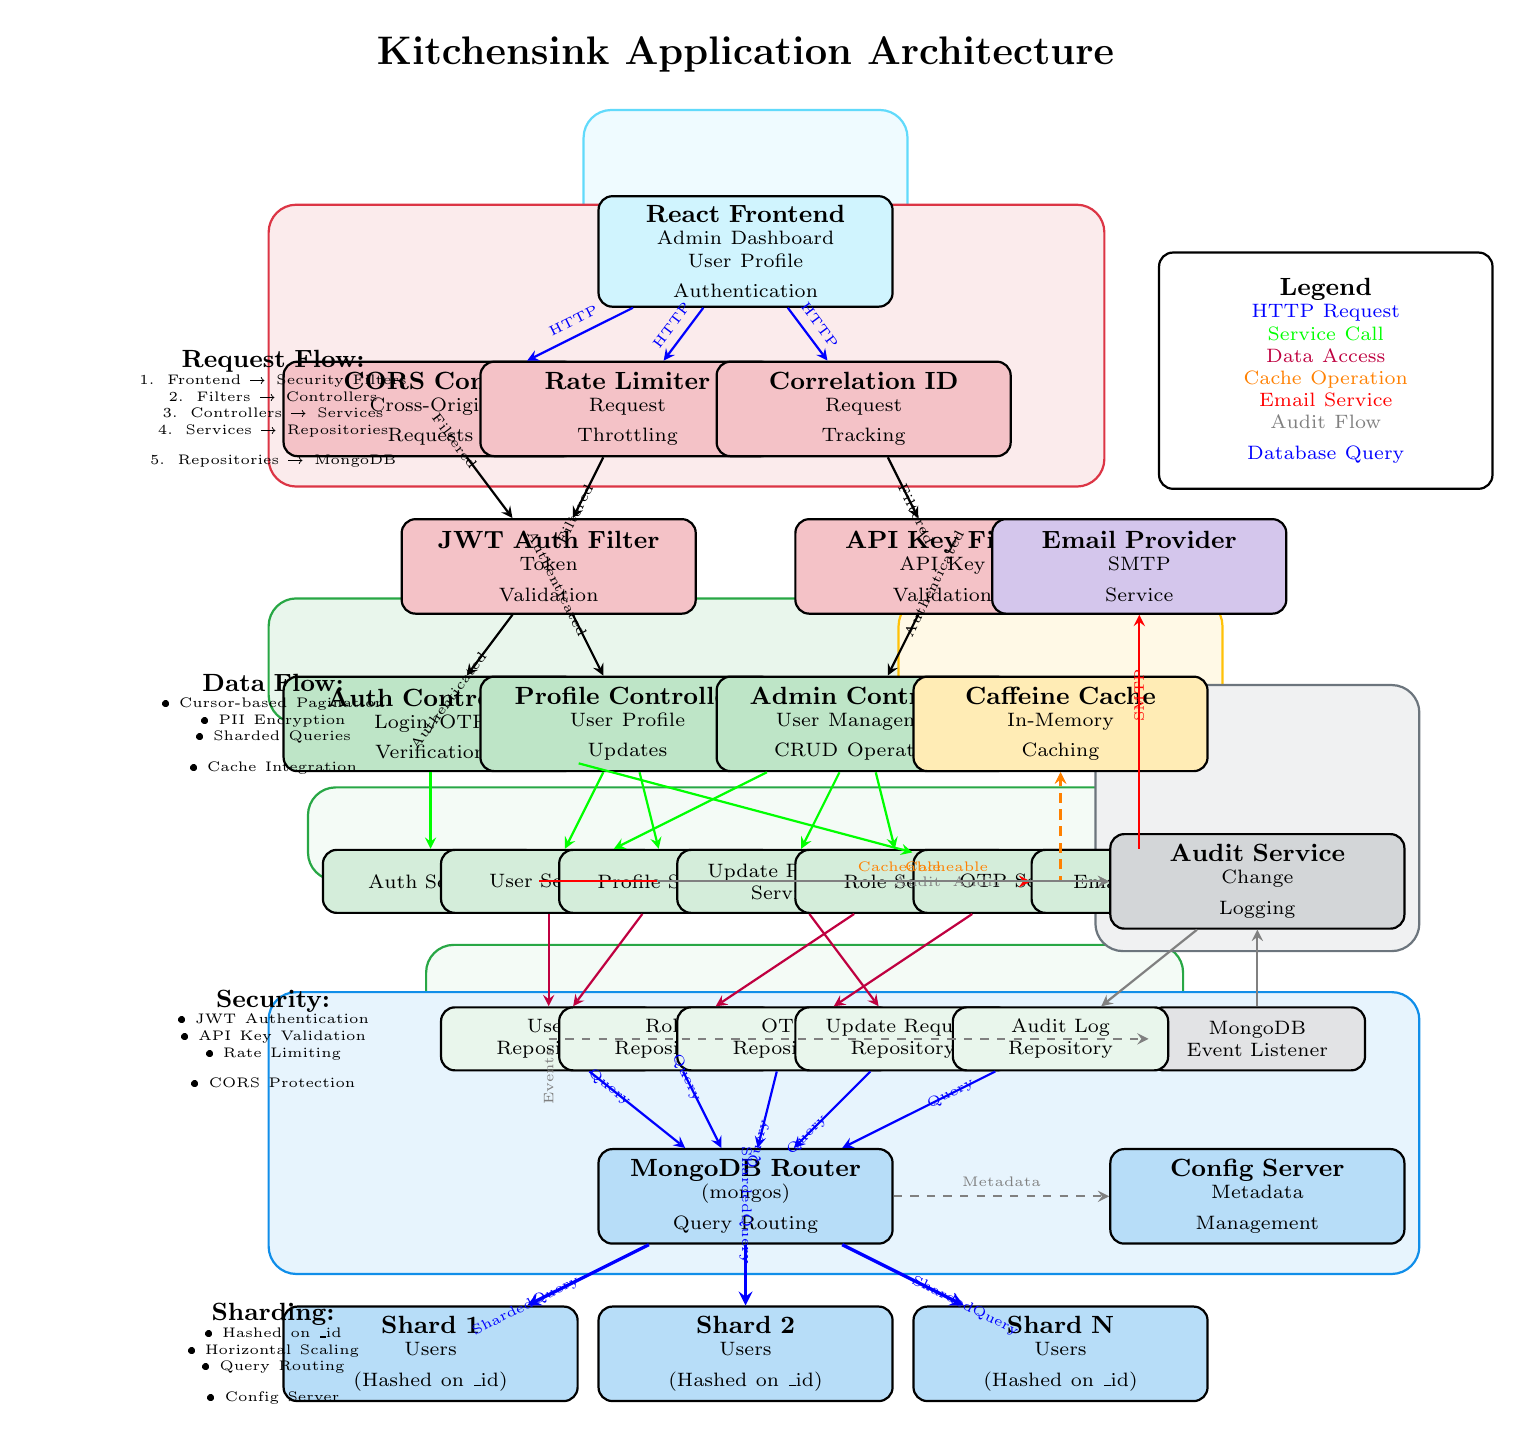
\begin{tikzpicture}[
    node distance=1.5cm and 2cm,
    box/.style={rectangle, rounded corners=5pt, draw=black, thick, text width=3.5cm, minimum height=1.2cm, text centered, font=\small},
    component/.style={rectangle, rounded corners=5pt, draw=black, thick, text width=2.5cm, minimum height=0.8cm, text centered, font=\scriptsize},
    arrow/.style={->, >=stealth, thick},
    label/.style={font=\tiny, above, sloped}
]

% ========== FRONTEND LAYER ==========
\node[box, fill=frontend!30] (react) at (0,8) {\textbf{React Frontend}\\
    \scriptsize Admin Dashboard\\
    \scriptsize User Profile\\
    \scriptsize Authentication};

% ========== SECURITY LAYER ==========
\node[box, fill=security!30] (cors) at (-4,6) {\textbf{CORS Config}\\
    \scriptsize Cross-Origin\\
    \scriptsize Requests};

\node[box, fill=security!30] (rateLimit) at (-1.5,6) {\textbf{Rate Limiter}\\
    \scriptsize Request\\
    \scriptsize Throttling};

\node[box, fill=security!30] (correlation) at (1.5,6) {\textbf{Correlation ID}\\
    \scriptsize Request\\
    \scriptsize Tracking};

\node[box, fill=security!30] (jwtAuth) at (-2.5,4) {\textbf{JWT Auth Filter}\\
    \scriptsize Token\\
    \scriptsize Validation};

\node[box, fill=security!30] (apiKey) at (2.5,4) {\textbf{API Key Filter}\\
    \scriptsize API Key\\
    \scriptsize Validation};

% ========== CONTROLLER LAYER ==========
\node[box, fill=backend!30] (authController) at (-4,2) {\textbf{Auth Controller}\\
    \scriptsize Login/OTP\\
    \scriptsize Verification};

\node[box, fill=backend!30] (profileController) at (-1.5,2) {\textbf{Profile Controller}\\
    \scriptsize User Profile\\
    \scriptsize Updates};

\node[box, fill=backend!30] (adminController) at (1.5,2) {\textbf{Admin Controller}\\
    \scriptsize User Management\\
    \scriptsize CRUD Operations};

% ========== SERVICE LAYER ==========
\node[component, fill=backend!20] (authService) at (-4,0) {Auth Service};
\node[component, fill=backend!20] (userService) at (-2.5,0) {User Service};
\node[component, fill=backend!20] (profileService) at (-1,0) {Profile Service};
\node[component, fill=backend!20] (updateService) at (0.5,0) {Update Request\\
    Service};
\node[component, fill=backend!20] (roleService) at (2,0) {Role Service};
\node[component, fill=backend!20] (otpService) at (3.5,0) {OTP Service};
\node[component, fill=backend!20] (emailService) at (5,0) {Email Service};

% ========== CACHE LAYER ==========
\node[box, fill=cache!30] (cache) at (4,2) {\textbf{Caffeine Cache}\\
    \scriptsize In-Memory\\
    \scriptsize Caching};

% ========== AUDIT LAYER ==========
\node[box, fill=audit!30] (auditService) at (6.5,0) {\textbf{Audit Service}\\
    \scriptsize Change\\
    \scriptsize Logging};

\node[component, fill=audit!20] (auditListener) at (6.5,-2) {MongoDB\\
    Event Listener};

% ========== DATABASE LAYER ==========
\node[box, fill=database!30] (mongos) at (0,-4) {\textbf{MongoDB Router}\\
    \scriptsize (mongos)\\
    \scriptsize Query Routing};

\node[box, fill=database!30] (shard1) at (-4,-6) {\textbf{Shard 1}\\
    \scriptsize Users\\
    \scriptsize (Hashed on \_id)};

\node[box, fill=database!30] (shard2) at (0,-6) {\textbf{Shard 2}\\
    \scriptsize Users\\
    \scriptsize (Hashed on \_id)};

\node[box, fill=database!30] (shard3) at (4,-6) {\textbf{Shard N}\\
    \scriptsize Users\\
    \scriptsize (Hashed on \_id)};

\node[box, fill=database!30] (configServer) at (6.5,-4) {\textbf{Config Server}\\
    \scriptsize Metadata\\
    \scriptsize Management};

% ========== EXTERNAL SERVICES ==========
\node[box, fill=external!30] (emailProvider) at (5,4) {\textbf{Email Provider}\\
    \scriptsize SMTP\\
    \scriptsize Service};

% ========== REPOSITORY LAYER ==========
\node[component, fill=backend!10] (userRepo) at (-2.5,-2) {User\\
    Repository};
\node[component, fill=backend!10] (roleRepo) at (-1,-2) {Role\\
    Repository};
\node[component, fill=backend!10] (otpRepo) at (0.5,-2) {OTP\\
    Repository};
\node[component, fill=backend!10] (updateRepo) at (2,-2) {Update Request\\
    Repository};
\node[component, fill=backend!10] (auditRepo) at (4,-2) {Audit Log\\
    Repository};

% ========== ARROWS - FRONTEND TO SECURITY ==========
\draw[arrow, color=blue] (react) -- (cors) node[label, pos=0.5] {HTTP};
\draw[arrow, color=blue] (react) -- (rateLimit) node[label, pos=0.5] {HTTP};
\draw[arrow, color=blue] (react) -- (correlation) node[label, pos=0.5] {HTTP};

% ========== ARROWS - SECURITY TO CONTROLLERS ==========
\draw[arrow, color=black] (cors) -- (jwtAuth) node[label, pos=0.3, left] {Filtered};
\draw[arrow, color=black] (rateLimit) -- (jwtAuth) node[label, pos=0.3, left] {Filtered};
\draw[arrow, color=black] (correlation) -- (apiKey) node[label, pos=0.3, right] {Filtered};

\draw[arrow, color=black] (jwtAuth) -- (authController) node[label, pos=0.5, left] {Authenticated};
\draw[arrow, color=black] (jwtAuth) -- (profileController) node[label, pos=0.5, left] {Authenticated};
\draw[arrow, color=black] (apiKey) -- (adminController) node[label, pos=0.5, right] {Authenticated};

% ========== ARROWS - CONTROLLERS TO SERVICES ==========
\draw[arrow, color=green] (authController) -- (authService);
\draw[arrow, color=green] (authController) -- (otpService);
\draw[arrow, color=green] (profileController) -- (profileService);
\draw[arrow, color=green] (profileController) -- (userService);
\draw[arrow, color=green] (adminController) -- (userService);
\draw[arrow, color=green] (adminController) -- (updateService);
\draw[arrow, color=green] (adminController) -- (roleService);

% ========== ARROWS - SERVICES TO REPOSITORIES ==========
\draw[arrow, color=purple] (userService) -- (userRepo);
\draw[arrow, color=purple] (roleService) -- (roleRepo);
\draw[arrow, color=purple] (otpService) -- (otpRepo);
\draw[arrow, color=purple] (updateService) -- (updateRepo);
\draw[arrow, color=purple] (profileService) -- (userRepo);

% ========== ARROWS - SERVICES TO CACHE ==========
\draw[arrow, color=orange, dashed] (userService) -| (cache) node[label, pos=0.3, above] {Cacheable};
\draw[arrow, color=orange, dashed] (profileService) -| (cache) node[label, pos=0.3, above] {Cacheable};

% ========== ARROWS - SERVICES TO EMAIL ==========
\draw[arrow, color=red] (authService) -- (emailService);
\draw[arrow, color=red] (userService) -- (emailService);
\draw[arrow, color=red] (emailService) -- (emailProvider) node[label, pos=0.5, right] {SMTP};

% ========== ARROWS - REPOSITORIES TO MONGODB ==========
\draw[arrow, color=blue, thick] (userRepo) -- (mongos) node[label, pos=0.5, left] {Query};
\draw[arrow, color=blue, thick] (roleRepo) -- (mongos) node[label, pos=0.5, left] {Query};
\draw[arrow, color=blue, thick] (otpRepo) -- (mongos) node[label, pos=0.5, left] {Query};
\draw[arrow, color=blue, thick] (updateRepo) -- (mongos) node[label, pos=0.5, left] {Query};
\draw[arrow, color=blue, thick] (auditRepo) -- (mongos) node[label, pos=0.5, right] {Query};

% ========== ARROWS - MONGOS TO SHARDS ==========
\draw[arrow, color=blue, very thick] (mongos) -- (shard1) node[label, pos=0.5, left] {Sharded\\
    Query};
\draw[arrow, color=blue, very thick] (mongos) -- (shard2) node[label, pos=0.5, left] {Sharded\\
    Query};
\draw[arrow, color=blue, very thick] (mongos) -- (shard3) node[label, pos=0.5, right] {Sharded\\
    Query};

% ========== ARROWS - MONGOS TO CONFIG ==========
\draw[arrow, color=gray, dashed] (mongos) -- (configServer) node[label, pos=0.5, above] {Metadata};

% ========== ARROWS - AUDIT FLOW ==========
\draw[arrow, color=gray] (userService) -- (auditService) node[label, pos=0.5, right] {Audit};
\draw[arrow, color=gray] (profileService) -- (auditService) node[label, pos=0.5, right] {Audit};
\draw[arrow, color=gray] (auditService) -- (auditRepo);
\draw[arrow, color=gray, dashed] (userRepo) |- (auditListener) node[label, pos=0.3, left] {Events};
\draw[arrow, color=gray] (auditListener) -- (auditService);

% ========== BACKGROUND BOXES ==========
\begin{scope}[on background layer]
    \node[fit=(react), fill=frontend!10, draw=frontend, thick, rounded corners=10pt, inner sep=5pt, label={[font=\small, anchor=south west]south west:Frontend Layer}] {};
    
    \node[fit=(cors)(rateLimit)(correlation)(jwtAuth)(apiKey), fill=security!10, draw=security, thick, rounded corners=10pt, inner sep=5pt, label={[font=\small, anchor=south west]south west:Security Layer}] {};
    
    \node[fit=(authController)(profileController)(adminController), fill=backend!10, draw=backend, thick, rounded corners=10pt, inner sep=5pt, label={[font=\small, anchor=south west]south west:Controller Layer}] {};
    
    \node[fit=(authService)(userService)(profileService)(updateService)(roleService)(otpService)(emailService), fill=backend!5, draw=backend, thick, rounded corners=10pt, inner sep=5pt, label={[font=\small, anchor=south west]south west:Service Layer}] {};
    
    \node[fit=(userRepo)(roleRepo)(otpRepo)(updateRepo)(auditRepo), fill=backend!5, draw=backend, thick, rounded corners=10pt, inner sep=5pt, label={[font=\small, anchor=south west]south west:Repository Layer}] {};
    
    \node[fit=(mongos)(shard1)(shard2)(shard3)(configServer), fill=database!10, draw=database, thick, rounded corners=10pt, inner sep=5pt, label={[font=\small, anchor=south west]south west:Database Layer (Sharded)}] {};
    
    \node[fit=(cache), fill=cache!10, draw=cache, thick, rounded corners=10pt, inner sep=5pt, label={[font=\small, anchor=south west]south west:Caching}] {};
    
    \node[fit=(auditService)(auditListener), fill=audit!10, draw=audit, thick, rounded corners=10pt, inner sep=5pt, label={[font=\small, anchor=south west]south west:Auditing}] {};
\end{scope}

% ========== LEGEND ==========
\node[box, fill=white, text width=4cm, minimum height=3cm, anchor=north east] (legend) at (9.5,8) {\textbf{Legend}\\
    \scriptsize \textcolor{blue}{HTTP Request}\\
    \scriptsize \textcolor{green}{Service Call}\\
    \scriptsize \textcolor{purple}{Data Access}\\
    \scriptsize \textcolor{orange}{Cache Operation}\\
    \scriptsize \textcolor{red}{Email Service}\\
    \scriptsize \textcolor{gray}{Audit Flow}\\
    \scriptsize \textcolor{blue}{Database Query}};

% ========== TITLE ==========
\node[font=\Large\bfseries] (title) at (0,10.5) {Kitchensink Application Architecture};

% ========== FLOW LABELS ==========
\node[font=\small, text width=6cm, align=center] (flow1) at (-6,6) {\textbf{Request Flow:}\\
    \tiny 1. Frontend → Security Filters\\
    \tiny 2. Filters → Controllers\\
    \tiny 3. Controllers → Services\\
    \tiny 4. Services → Repositories\\
    \tiny 5. Repositories → MongoDB};

\node[font=\small, text width=6cm, align=center] (flow2) at (-6,2) {\textbf{Data Flow:}\\
    \tiny • Cursor-based Pagination\\
    \tiny • PII Encryption\\
    \tiny • Sharded Queries\\
    \tiny • Cache Integration};

\node[font=\small, text width=6cm, align=center] (flow3) at (-6,-2) {\textbf{Security:}\\
    \tiny • JWT Authentication\\
    \tiny • API Key Validation\\
    \tiny • Rate Limiting\\
    \tiny • CORS Protection};

\node[font=\small, text width=6cm, align=center] (flow4) at (-6,-6) {\textbf{Sharding:}\\
    \tiny • Hashed on \_id\\
    \tiny • Horizontal Scaling\\
    \tiny • Query Routing\\
    \tiny • Config Server};

\end{tikzpicture}
\end{document}

